\documentclass[12pt]{article}
\usepackage{graphicx}
\usepackage{hyperref}
\graphicspath{{Img/}}
\usepackage[a4paper, total={6.5in, 9.6in}]{geometry}
\title{Controlling Cursor using Hand Gesture Recognition\\MLP-11}
\author{Rishikesh Dhurde (B-48), Ritik Ragit (B-49)}
\begin{document}
\maketitle
\section{Abstract}
Our main objective of doing this project is to build an application which can recognize hand gestures and we are trying to give a more personal and interactive touch to interface by using the hand gesture control and it can be used to perform functions of mouse cursor to virtually control a computer.

\section{Introduction}
Computer technology has grown tremendously over the past few years and has became an important part of our everyday life. The basic computer accessory for Human to Computer Interaction is the mouse. The regular mouse is not appropriate for Human to Computer Interaction in some real life situations, such as with the Human Robot Interaction. There have been many researches on alternative methods to the computer mouse for Human to Computer Interaction. The most natural and intuitive technique for Human to Computer Interaction, that is a viable replacement for the computer mouse is with the use of hand gestures. This project is therefore aimed at investigating and developing a Computer Control system using hand gestures.
\\
Most laptops today are equipped with webcams, which have recently been used insecurity applications utilizing face recognition. In order to harness the full potential of a webcam, it can be used for vision based Computer Control, which would effectively eliminate the need for a computer mouse or mouse pad. The usefulness of a webcam can also be greatly extended to other Human to Computer Interaction application such as a sign language database or motion controller.\cite{2}


\section{Related Work}
1.Hand Recognition and Gesture Control Using a Laptop Web Camera.\\
\url{https://web.stanford.edu/class/cs231a/prev_projects_2016/CS231A_Project_Final.pdf}\\
In this paper the authors made a hand recognition and gesture control system using a laptop web-camera. They tried three hand segmentation methods- \\
1.Canny Edge detection(This allowed for color contrasts between
the hand and the background, which could be interpreted
as edges).\\
2.Background Subtraction(this involves having the program
read multiple frames and subtracting the aggregate values
from future frames).\\
3.Calibration and Thresholding(this method has the potential to be fairly accurate in segmenting the hand, it turned out to be very sensitive to the environment).\\
\\
2.OBJECT DETECTION AND IDENTIFICATION A Project Report\\
\url{https://www.researchgate.net/publication 337464355}\\ 
In this paper the author has briefly discussed about the object detection concepts. This paper covers about R-CNN, as it's a family of techniques for addressing object recognition tasks and designed for model performances. YOLO is another class of technique for object recognition implemented for real-time use. This paper also covers comparison of speed and accuracy between R-CNN, Fast R-CNN, Faster R-CNN, YOLO and SSD. \\ 
\\
3.Real-time Hand-Detection using Neural Networks (SSD) on Tensorflow.\\
\url{https://github.com/victordibia/handtracking}\\
In this repository a model is used to train a hand detector using Tensorflow (Object Detection API). The goal of this repo/post is to demonstrate how neural networks can be applied to the (hard) problem of tracking hands (egocentric and other views). In this model single shot detector is used, SSD only needs an input image and ground truth boxes for each object during training.\cite{1}

\section{Dataset and Features}
We have made our own data set of images. First we clicked about 600 different images of multiple hand gestures in the different lighting conditions and in daily life environment. After this we labelled all the images using the labelImg tool. After the labelling we get an XML file for each image, this XML file contains details about the bounding box, the class that we have created with in that image. Here we have divided the images in the ratio of 80:20. 80 percent of images for training and 20 percent for the testing of the model. Then we generated the csv file from the obtained xml files, for training and testing of the dataset. Then we used tensorflow object detection model and configured it with its particular configuration file to train this model. After this we started training up the model, using Google Collab by utilising it's GPU. we trained this model for more than 100000 iterations and having very low loss of about 0.1. Then we generated the inference graph for using the model. That's the trained model.
\begin{figure}[h]
\centering
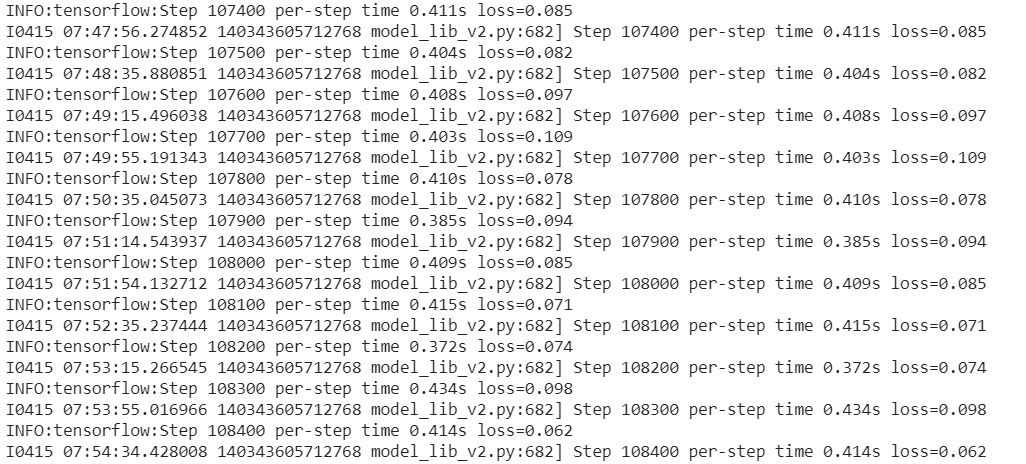
\includegraphics[scale=0.48]{training.PNG}
\caption{Training of Model}
\label{training.PNG}
\end{figure}

\section{Methods}
We are trying deep learning to implement this recognition system. By using  convolutional neural network, we will train the system by adding multiple different images of hand and different gestures and set the output as per the gestures to perform the basic tasks of the mouse.\\
\\
We have used deep learning because the data we are using to train the algorithm is already labeled with correct answers(operations). And we will try to identify different hand gestures, which are already trained on a dataset of images that are properly labeled with the hand sign operations.\\
\\
So for this project we have chosen the Object Detection Algorithm i.e. Single Shot Detector(SSD). SSD has a decent balance between the accuracy and speed. SSD runs a convolutional network on input image only once and calculates it's feature map(like in our case different fingers). VGG-16 Network is used to extract feature maps in the SSD. An SSD makes 8732 predictions(bounding boxes) for every single object. SSD willcheck the confidence score of each box and will pick the top 200 predictions per image. For training of SSD we should have images with ground truth boxes, for each object. Apart from these multiple default boxes of different sizes and aspect ratios are across the image. This process will help us finding the box that overlap the ground truth bounding box. We will check this by finding Intersection over Union(IOU) i.e. (Area of Overlap)/(Area of Union), with the help of IOU we are finding a box having highest overlap and that box is finalized as output out of the 8732 boxes. \\
\begin{figure}[h]
\centering
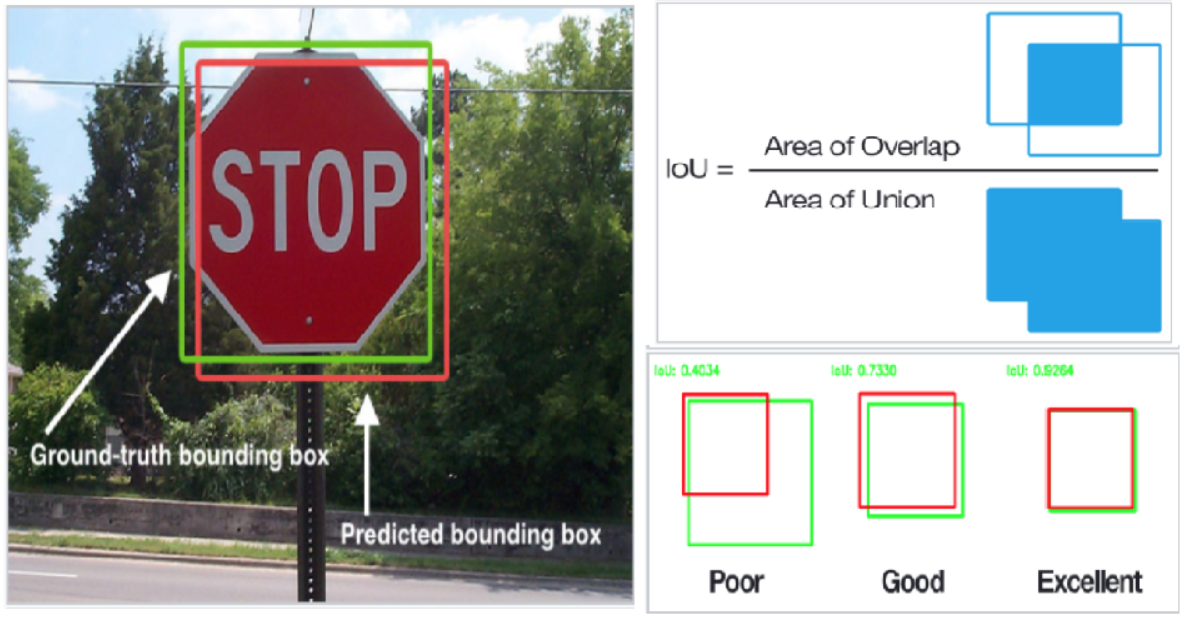
\includegraphics[scale=0.5]{GTB_IOU.PNG}
\caption{Bounding box process}
\label{GTB_IOU.PNG}
\cite{5}
\end{figure}

\section{Experiments/Results/Discussion}
We have chosen the state of art model from tensorflow zoo. For this model we have chosen the learning rate to be 0.0001 and number of epochs are more than 100000, we have chosen such small learning rate because we are having less number of images. Batch size of 4 is selected for this model, because we are not having GPU on our system, so we performed the training on Google Collab.\\
\\
On SSD model we got the maximum accuracy. Before SSD we have tried the YOLOv3, but here we are not getting the proper accuracy, and sometime it simply did not recognized the hand gestures. For YOLO detection is like a  regression problem which takes input image and learns about the class probabilities and bounding box coordinates. If accuracy is not a concern and have to train the model super fast then YOLO is the best.\cite{4}\\
\\
\begin{figure}[h]
\centering
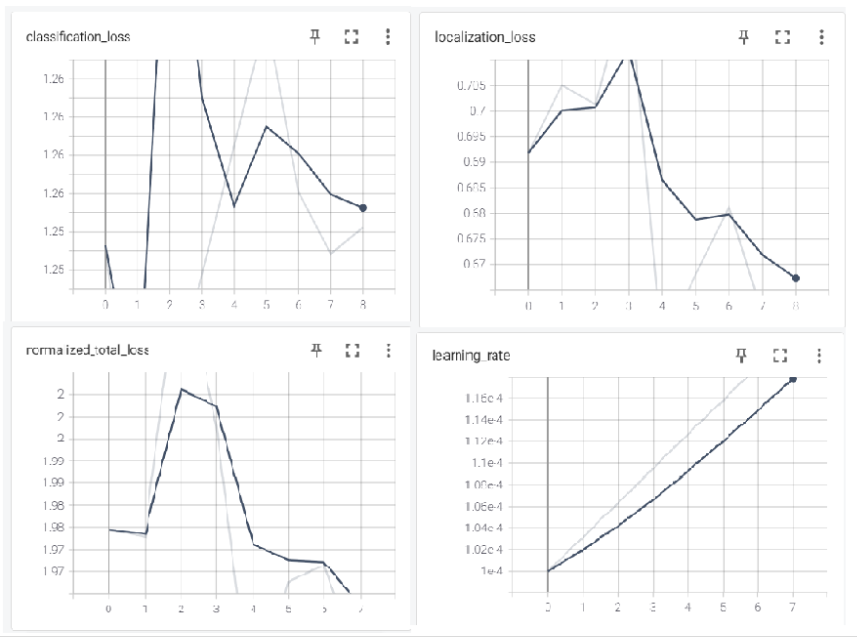
\includegraphics[scale=0.55]{Graph.PNG}
\caption{Graph of Accuracy and Loss}
\label{Graph.PNG}
\end{figure}
\\
\begin{table}[ht]
\centering % used for centering table
\begin{tabular}{|c|c|c|}
\hline % inserts single horizontal line
n=125 & Predicted:NO & Predicted:Yes \\ % inserting body of the table
\hline
Actual:No & 1 & 2 \\
\hline
Actual:Yes & 3 & 119 \\ [1ex] % [1ex] adds vertical space
\hline %inserts single line
\end{tabular}
\label{table:nonlin} % is used to refer this table in the text
\caption{Confusion Matrix}
\end{table}
\\
Accuracy = (No. of Correct Prediction)/(Total No. of input Samples)\\
Accuracy = 120/125 = 96 percent.\\
\\
Precision = (Total Positive)/(Total Positive+False Positive)\\
Precision = 119/121 = 98.34 percent.\\
\\
We have overviewed other  object detection algorithms also:\\
\\
1.Region-based Convolutional Neural Network(R-CNN): CNN are slow and computationally expensive, so R-CNN solves this problem by using an object proposal algorithm called selective search which reduces number of bounding boxes that are fed to the classifier.\cite{4}\\
\\
2.Fast R-CNN: It uses a simple back propagation calculation. Fast-RCNN added the bounding box regression to the neural network training itself. So the network has two heads classification head and bounding box regression head.\cite{4}\\
\\
3.Faster R-CNN: Well Faster RCNN is similar to Fast R-CNN, but it replaces selective search with a very small convolutional  network called Region Proposal Network to generate regions of Interests.\cite{4}
\begin{figure}[h]
\centering
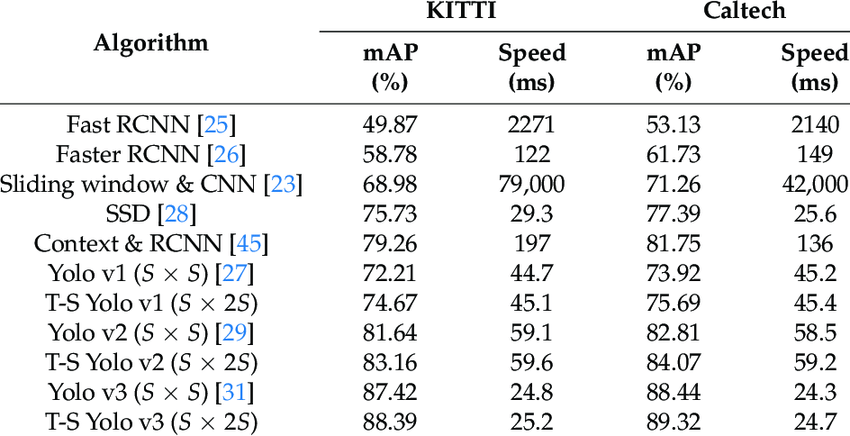
\includegraphics[scale=0.4]{Comparison.PNG}
\caption{Comparison between different object detection models}
\label{Comparison.PNG}
\cite{6}
\end{figure}

\section{Conclusion/Future Work}
We have tested our dataset using two object detection algorithm i.e. YOLO object detection model and SSD, and came to conclusion that SSD is suitable for our problem and dataset. YOLO was fast to train but we did not achieved the required accuracy. With SSD it took a lot of time to train the dataset but the accuracy was also appreciable.\\
\\
While implementing this project we faced many issues for dependencies of libraries, at the time of training as we don't have GPU in our device. But overall it was fun in implementing a hand gesture gestures recognition system from our own dataset.\\
\\
If we had more time, more members and more computational resources try to implement this on more object detection algorithms. We will try to increase accuracy and precision of the model, to smoothly control the cursor using hand gestures. And also try to increase our dataset for better optimization.
\\
\\
\\
\\
\section{Contributions}
RISHIKESH DHURDE (B-48)- Making of dataset, Writing and compiling report, Code writing and experimentation.\\
\\
RITIK RAGIT (B-49)- Code research, writing and debugging, Finding relative work and content.\\
\\
"For this project we had taken help and advise from my friend MR. TANUJ KAMDE."


\section{References/Bibliography}
\begin{thebibliography}{99}
\hypersetup{colorlinks=true,linkcolor=blue,filecolor=magenta,urlcolor=cyan,pdftitle={overleaf Example},bookmarks=true,pdfpagemode=FullScreen}

\bibitem{1}
\url{https://github.com/victordibia/handtracking}
\bibitem{2}
\url{https://michigansciencecenter.net/computer-technology-has-tremendously-grown-over-the-past-decade-and-has-become-a-necessary-part-of-everyday-live/}
\bibitem{3}
\url{https://www.researchgate.net/figure/SSD-framework-a-SSD-only-needs-an-input-image-and-ground-truth-boxes-for-each-object_fig1_286513835}
\bibitem{4}
\url{https://cv-tricks.com/object-detection/faster-r-cnn-yolo-ssd/}
\bibitem{5}
\url{https://www.pyimagesearch.com/2016/11/07/intersection-over-union-iou-for-object-detection/}
\bibitem{6}
\url{https://www.researchgate.net/figure/Detection-accuracy-and-speed-of-all-lane-detection-algorithms-on-KITTI-and-Caltech_tbl1_329475183}
\end{thebibliography}
\section{Git Hub Link}
\url{https://github.com/RishikeshDhurde/MLP-11.git}
\end{document}

